\begin{figure*}
	\centering
	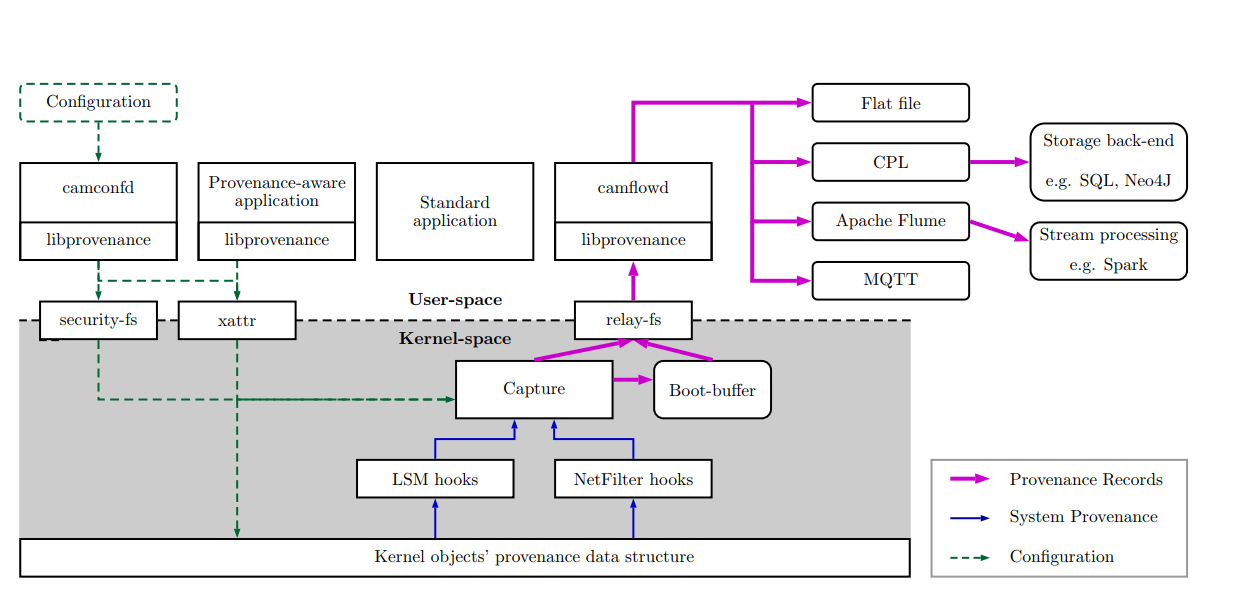
\includegraphics[width=0.7\linewidth]{camflow}
	\caption[Architecture overview]{Camflow architure}
	\label{fig:camflow}
\end{figure*}
\begin{figure}
	\centering
	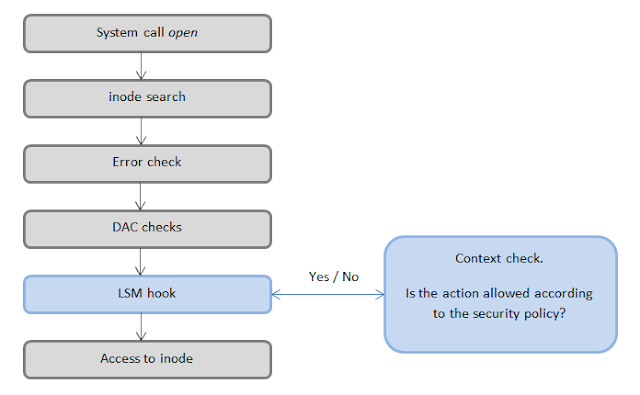
\includegraphics[width=0.7\linewidth]{LSM-hook}
	\caption[LSM hook]{LSM hook working for system call "open"}
	\label{fig:lsm-hook}
\end{figure}


\label{Introduction}
\section{LSMs and LSM hooks}
Though we have introduced what a Linux Security Module(LSM) means, we will discuss it in a little more detail. The Linux Security Module (LSM) framework provides a mechanism for various security checks to be hooked by new kernel extensions. The name “module” is a bit of a misnomer since these extensions are not actually loadable kernel modules. Instead, they are selectable at build-time via CONFIG\_DEFAULT\_SECURITY and can be overridden at boot-time via the "security=..." kernel command line argument, in the case where multiple LSMs were built into a given kernel.
\subsection{LSMs and policies}
The primary users of the LSM interface are Mandatory Access Control (MAC) extensions which provide a comprehensive security policy. Examples include SELinux, Smack, Tomoyo, and AppArmor. In addition to the larger MAC extensions, other extensions can be built using the LSM to provide specific changes to system operation when these tweaks are not available in the core functionality of Linux itself.
\subsection{Types of LSMs}
Without a specific LSM built into the kernel, the default LSM will be the Linux capabilities system. Most LSMs choose to extend the capabilities system, building their checks on top of the defined capability hooks.
\vskip 0.1in
The different types of Linux Security Modules are listed in Table 1. The entire list of the LSMs can be found by reading \textit{/sys/kernel/security/lsm}. The Table 1 reflects the order in which checks are made. The capability module is always first, followed by "minor" e.g. Yama) and then the one “major” module (e.g. SELinux) if there is one configured. This information will help us in understanding the next part of our research. 
\subsection{LSM Hooks}
In order to explain how a LSM hook works, we show an example in Fig 4. We take system call open as an example. We can see in Fig 4 that just before the kernel addresses an internal object, a check function provided by LSM is called. Hence, LSM allows the modules to understand wheather subject S is allowed to perform an action OP over kernel's internal object OBJ.


\begin{table}[ht]
	\caption{Linux Security Modules}
	\centering
	\begin{tabular}{c}
		\hline\hline 
		Different LSMs \\
		\hline
		AppArmor \\
		LoadPin  \\
		SELinux  \\
		Smack   \\
		TOMOYO \\
		Yama \\
	\end{tabular}	
\end{table}


\section{Modelling the system calls causing flows}
The analysis proposed relies on the C compiler from the
Gnu Compilers Collection [23], used to compile the Linux
kernel

\subsection{Control flow graphs}
The analysis technique we use if has been proposed by Georget et al. () for a subset of the system calls. It's a four step methodology which relies on the C compiler from the Gnu Compilers Collection(21). 

\begin{enumerate}
	\item The model designed by Georget to represent system calls and their execution paths does not describe the C source code. They instead use an internal representation called GIMPLE[]. 
	\item Each system call is represented by a control flow graph (CFG).
	\item The paths in these graphs model the execution paths in the program as defined by the classical graph theory[].
	\item The system calls are analysed one at a time. 
	\item Each system call contains multiple functions. These functions are inlined into the system calls to reduce the analysis to intra-procedural case. 
	\item Finally, in the CFGs, two kinds of nodes are marked: the nodes which correspond to the LSM hooks and the nodes which correspond to operation which generate the flows. 
	\end{enumerate}

\subsection{Constraints in modelling}
In the CFGs which we construct , a node is not a basic block but a simple GIMPLE instruction. The analysis methodology does not deal with all expressions and variables of the language. Another reason for the same is that usage of floating-point values is explicitly prohibited in the Linux code. Variables representing structures or unions are also not handled when they involve pointer arithmetic. Global or volatile variables are also not handled, since they can have an arbitrary value at any point in the execution. Ignoring some variables does not hinder the soundness of
our approach: less impossible paths might be detected as such but
we never declare as impossible a possible path. A path in the CFG is said to be impossible when any execution
that would follow it would enter in an impossible state. For example,
a path including two conditional branching with incompatible
conditions would require a Boolean expression to be both true and
false at the same time. 
\vskip 0.1in
There are powerful static analysers available such as Blast(24) available. However, for our need to ensure the complete mediation property, we don't need a framework which deals with complex types and data structures. The mediation property which we have described in the previous section despite introducing the above mentioned constraints provides us with precise modelling.

\section{Static analysis on paths}
The goal of static analysis is to verify that information flow goes through a LSM hook or that it is impossible. In order to do so, we need to find the information flows for any CFG representing a system call.

\subsection{Verifying complete mediation}
We consider the set \textit{Paths} of all paths in a CFG.We introduce two particular subsets in this:(1) the set
Paths$_{flows}$  of paths starting at the initial node of the CFG and
ending at one node generating an information flow; and (2) the
set Paths$_{LSM}$  of paths having a node corresponding to a LSM
hook. The placement of the hooks would be obviously correct
if we could prove that Paths$_{flows}$ $\subseteq$ Paths$_{LSM}$ . However, as
we will see, this is not the case. Pf =  Paths$_{flows}$ \ Paths$_{LSM}$. The sets involved in the analysis are shown diagrammatically in Fig. 5.
represents the set of paths that may be problematic.
\vskip 0.1in
As explained earlier, some paths in Paths$_{flows}$  are actually
impossible, and therefore even if there are no LSM hooks
in them, they are not actually problematic. Recall that an
impossible path is a path that does not correspond to a possible
execution. The objective of our analysis is thus to verify that
P$_f$ $\subseteq$ I where I $\subseteq$ Paths is the set of impossible paths in
the CFG.
\vskip 0.1in
The property which we are looking to verify is the complete mediation property. Explaining the entire proof is out of scope of this paper. Hence, we state the entire property here.
\vskip 0.1in
\subsubsection[Property 1 (Complete Mediation)]{Property 1 (Complete Mediation):}
Complete mediation holds iff: P$_f$ $\subseteq$ I, i.e. all the execution
paths that perform an information flow and are not controlled
by the information flow monitor since they do not contain a
LSM hook are impossible according to the static analysis.
\begin{figure}
	\centering
	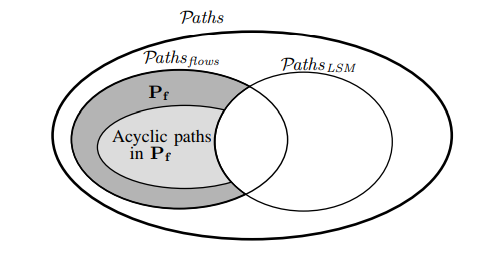
\includegraphics[width=0.7\linewidth]{Sets-involved}
	\caption[Sets involved in analysis]{Sets involved in analysis}
	\label{fig:sets-involved}
\end{figure}

\subsection{Soundness of proofs}
The soundness of our analysis is stated as follows.
\vskip 0.1in
\subsubsection{Proposition 1 (Soundness)}
For each path p in a CFG, for all concrete configurations $\theta_1$
and $\theta_2$, and all abstract configurations k$_1$ and k$_2$ such that
$\theta$1 →∗p
$\theta$2 and k1 ∗
p k2, we have θ1  k1 =⇒ θ2  k2.
